\begin{problema}
	Sea $N$ un proceso Poisson de par\'ametro $\lambda$ y sea $T_n$ el tiempo de su en\'esimo salto. 
	
	\begin{enumerate}
		\item[(i)]		[\ref{problema5_1:inciso1}] 
			Pruebe que condicionalmente a $T_2$, $T_1$ es uniforme en $[0,T_2]$.\pn
			
		\item[(ii)]		[\ref{problema5_1:inciso2}] 
			Pruebe que si $W_1$ y $W_2$  son  exponenciales de par\'ametro 
			$\lambda$  independientes entre si y de una variable uniforme $U$, 
			entonces $U\paren{W_1+W_2}$ es una variable aleatoria exponencial 
			de par\'ametro $\lambda$.\pn

		\item[(iii)]	[\ref{problema5_1:inciso3}] 
			Conjeture c\'omo se  generaliza lo anterior con $T_n$ y $T_1$.\pn

		\item[(iv)]		[\ref{problema5_1:inciso4}] 
			Escriba dos programas en Octave que simulen al proceso de Poisson 
			de par\'ametro $\lambda$ en el intervalo $[0,1]$. En uno utilizar\'a 
			s\'olo variables exponenciales y en el otro puede utilizar una 
			variable Poisson.\pn
	\end{enumerate}
\end{problema}

\begin{proof}
    \subsection{Inciso (i)} \label{problema5_1:inciso1}
    \emph{
	Pruebe que condicionalmente a $T_2$, $T_1$ es uniforme en $[0,T_2]$.
}

\afterstatement\pn

Por definición de proceso Poisson de parámetro $\lambda$, la distribución de los saltos $S_n$ es
exponencial de parámetro $\lambda$. Como $T_1 = S_1$ y $T_2 = S_1 + S_2$, entonces
$T_1  = S_1 \sim exp(\lambda) $ y  $T_2 - T_1 = S_2 \sim exp(\lambda)$.\pn

También por definición de proceso de Poisson, los saltos son independientes y por lo tanto
$T_1$ y $T_2 - T_1$ son independientes.\pn

Podemos dar su distribución conjunta como sigue:
\begin{align}
    f_{T_1, T_2 - T_1}(u, v)    &=  (\lambda e^{-\lambda u}) (\lambda e^{-\lambda v}) \indic_{\{ u > 0, v > 0 \}}   \\
                                &=  \lambda^2 e^{-\lambda (u + v)} \indic_{\{ u > 0, v > 0 \}}.
\end{align}

Hacemos el cambio de variable dado por la transformación lineal $l : (u, v-u) \longrightarrow (u, v)$.
La matriz asociada a esta transformación lineal tiene la forma

\[
    \left(
            \begin{array}{cc}
                    1   &   1   \\
                    0   &   1   \end{array}
    \right)
\]

cuyo determinante es $(1 \cdot 1) - (1 \cdot 0) = 1$ y por lo tanto tiene inversa (es fácil comprobar que $l^{-1}(u,v) = (u, v - u)$). 
Entonces, podemos escribir

\begin{align}
    f_{T_1, T_2}(u, v)      &=    f_{T_1, T_2 - T_1}(l^{-1}(u, v))                                      \\
                            &=    f_{T_1, T_2 - T_1}(u, v - u)                                          \\
                            &=    \lambda^2 e^{-\lambda (u + v - u)} \indic_{\{ u > 0, v - u > 0 \}}.   \\
                            &=    \lambda^2 e^{-\lambda (v)} \indic_{\{ v > u > 0 \}}.                    
\end{align}\pn

Ahora, $T_2 = (T_1) + (T_2 - T_1)$, de donde $T_2 \sim gamma(2, \lambda)$ y por lo tanto su función de densidad esta dada por

\begin{align}
    f_{T_2}(v) = \lambda^2 v e^{-\lambda v} \indic_{v \geq 0}.
\end{align}

Con todo esto, ahora podemos calcular la densidad condicional $f_{T_1 | T_2}$.

\begin{align}
    f_{T_1 | T_2}(u | v)    &=     \frac{f_{T_1 , T_2}(u, v)}{ f_{T_2}(v)}                                                                      \\
                            &=     \frac{\lambda^2 e^{-\lambda (v)} \indic_{\{ v > u > 0 \}}}{ \lambda^2 v e^{-\lambda v} \indic_{v \geq 0}}    \\
                            &=     \frac{ \indic_{\{ v > u > 0 \}}}{ v  \indic_{v \geq 0}}                                                      \\
                            &=     \frac{ \indic_{\{ v > u > 0 \}}}{v}.                                                      
\end{align}\pn

Y esto no es otra cosa que la distribución uniforme sobre $[0, v]$, es decir, la distribución uniforme sobre $[0, T_2]$.
    \newpage

    \subsection{Inciso (ii)} \label{problema5_1:inciso2}
    \emph{
	Pruebe que si $W_1$ y $W_2$  son  exponenciales de par\'ametro 
	$\lambda$  independientes entre si y de una variable uniforme $U$, 
	entonces $U\paren{W_1+W_2}$ es una variable aleatoria exponencial 
	de par\'ametro $\lambda$.
}

\afterstatement\pn
    \newpage

    \subsection{Inciso (iii)} \label{problema5_1:inciso3}
    \emph{
	Conjeture c\'omo se  generaliza lo anterior con $T_n$ y $T_1$.
}
	\newpage
	
    \subsection{Inciso (iv)} \label{problema5_1:inciso4}
    \emph{
	Escriba dos programas en Octave que simulen al proceso de Poisson 
	de par\'ametro $\lambda$ en el intervalo $[0,1]$. En uno utilizar\'a 
	s\'olo variables exponenciales y en el otro puede utilizar una 
	variable Poisson.
}

Utilizando variables de distribución exponencial para los 
saltos:\pn

\small
\texttt{
	\lstinputlisting[inputencoding=utf8]{tarea5/problema5_1/ProcesoPoissonConExponenciales.m}
}
\normalsize

A continuación una gráfica obtenida de ejecutar este código:\pn
\begin{center}
    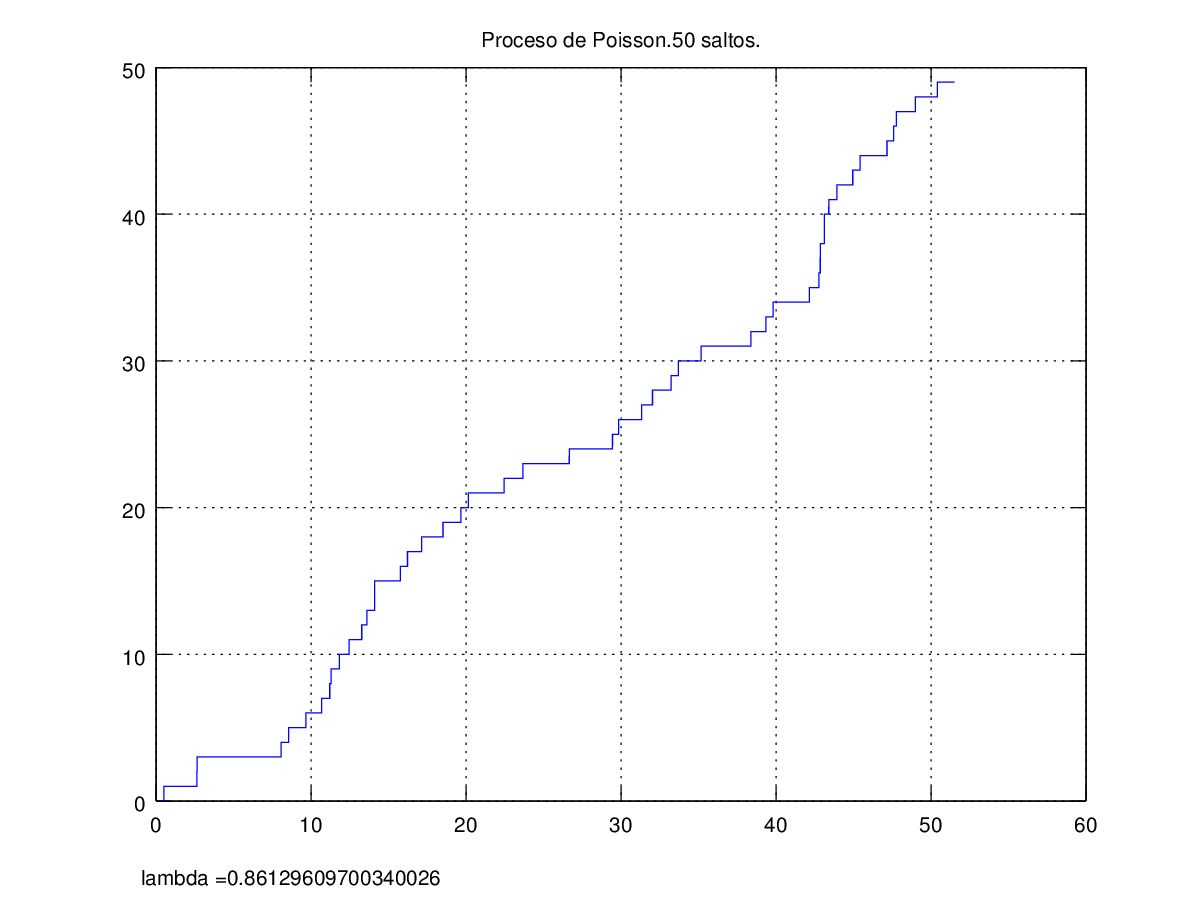
\includegraphics[width=8cm]{tarea5/problema5_1/ProcesoPoissonConExponenciales.png}
\end{center}

La implementación anterior fue hecha intentando representar el proceso de Poisson de parámetro
$\lambda$ durante los $50$ primeros saltos.

\newpage

Utilizando variables de distribución Poisson para determinar 
la cantidad de saltos hasta el tiempo $t$:\pn

\small
\texttt{
	\lstinputlisting[inputencoding=utf8]{tarea5/problema5_1/ProcesoPoissonConPoisson.m}
}
\normalsize

A continuación una gráfica obtenida de ejecutar este código:\pn

\begin{center}
    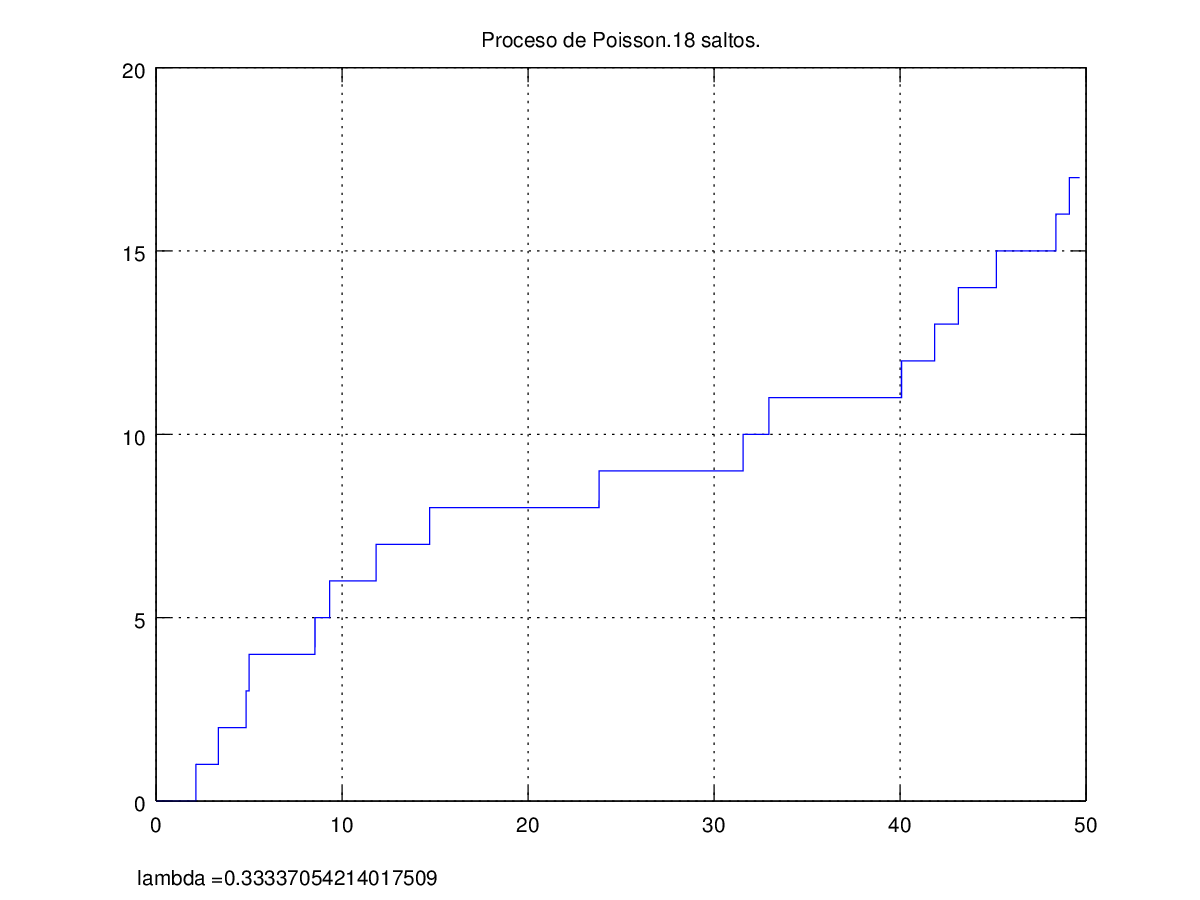
\includegraphics[width=8cm]{tarea5/problema5_1/ProcesoPoissonConPoisson.png}
\end{center}

A diferencia de la implementación anterior, esta vez intentamos representar el proceso de Poisson 
hasta un tiempo dado y no hasta un número de saltos dado. \pn

Como se puede apreciar, en esta última ejecución hasta el tiempo $50$ únicamente hubo $18$ saltos. 
A diferencia de que en la ejecución de la primera implementacción hubo $43$ saltos para el 
tiempo $50$. Cabe notar, que el parámetro lambda de la primera implementación era aproximadamente 
$0.915432$, mientras que el de la segunda a penas aproximadamente $0.333371$. Hay que recordar
que los ``holding times'' tienen distribución exponencial, tienden a ser más largos 
conforme $\lambda$ es más pequeño, y por lo tanto, entre más pequeño sea, habrá saltos con menos frecuencia.\pn

\textbf{Nota: } Para poder implementar esta versión del algoritmo se necesitó implementar
una función que se deduce del resultado de [\ref{problema5_1:inciso3}]. Esta parte está en el archivo con nombre
\texttt{t1\_dado\_tn\_rnd.m}. Esta función se usa para calcular los tiemos de salto y lo único
que hace es simular una variable aleatoria con la densidad del resultado de [\ref{problema5_1:inciso3}].
\end{proof}